\section{Overall Cooling Effectiveness (Requirement 4)}
\label{sec:effectiveness}

Requirements 2 and 3 compare useful cooling per kWh, $\eta=U/E$. Requirement 4 asks a different decision question: which installation balances cooling performance, visitor experience, energy and cost? The physical model and its outputs are retained; the decision criteria are expanded. This section organizes that extension. Cross-venue applications for Requirement 3 and empirical cost/experience inputs are still pending in this working draft.

\subsection{Four objectives with distinct roles}

For a common operating and accounting horizon $H$, compare the vector
\begin{equation}
 \min_s\big(\overline R_s,\ X_s,\ E_{s,H},\ C_{s,H}\big).
\label{eq:effectiveness-vector}
\end{equation}
Here $\overline R_s$ is mean remaining SET excess, so lower values indicate more complete thermal relief. $X_s$ represents non-thermal visitor-experience loss, such as the fraction reporting unacceptable equipment noise or obstructed access; it requires observations or surveys. SET-based thermal discomfort is not added to $X_s$ again. $E_{s,H}$ is energy use and $C_{s,H}$ is monetary cost over the same horizon. Because $U_s+R_s=R_0$ under a matched baseline, useful relief and residual discomfort are not treated as independent objectives, and $\eta$ is not added as a fifth objective.

A transparent cost model is
\begin{equation}
 C_{s,H}=\sum_k N_{s,k}\big(c_{k,H}^{\rm own}+c_{k,H}^{\rm maint}\big)
 +\pi_e E_{s,H}+\pi_w V_{s,H},
\label{eq:total-cost}
\end{equation}
where $N_{s,k}=\sum_zx_{zk}$, ownership and maintenance costs are allocated to $H$, $\pi_e,\pi_w$ are energy and water prices, and $V_{s,H}$ is make-up water including losses. All costs use one currency; $\pi_e$ is currency/kWh, $\pi_w$ is currency/m$^3$ and $V$ is m$^3$. Prices, ownership costs, water losses and experience data have not been supplied. We therefore retain these as inputs rather than inventing a calibrated cost or experience ranking. Energy represents a resource objective, while cost represents expenditure; the correlated quantities are not simply added with arbitrary equal weights.

\subsection{Service requirements and a conditional decision rule}

Let $q_s$ be person-time coverage, already used to account for exposure in Requirement 2. In this extension an operator may additionally require $q_s\ge q_{\min}$ and $\overline R_s\le R_{\max}$. For an electricity-priority policy, the earlier selection rule now belongs here:
\begin{equation}
 s^*=\arg\min_s E_{s,H}\quad\text{subject to}\quad
 \overline R_s\le R_{\max},\quad q_s\ge q_{\min},\quad
 X_s\le X_{\max},\quad C_{s,H}\le B_H.
\label{eq:effectiveness-selection}
\end{equation}
The bounds express stated service, experience and budget requirements, not universal SET safety limits. A cost-priority operator could instead minimize $C_{s,H}$ with an energy cap. If no priorities or bounds are specified, report nondominated choices for Eq.~\eqref{eq:effectiveness-vector}; no unique overall winner follows from efficiency alone.

\subsection{What the existing simulations demonstrate}

Across the same full set of 24 station candidates, A3 maximizes efficiency, while A36 delivers much wider direct service (Table~\ref{tab:efficiency-effectiveness}). These observations motivate the extension; they do not establish a complete effectiveness ranking.

\begin{table}[!ht]
\centering\small
\caption{Efficiency and service adequacy are different questions. Nominal two-hour simulations, with the same weather and passenger demand.}
\label{tab:efficiency-effectiveness}
\begin{tabular}{@{}lrrrr@{}}
\toprule
Plan & $\eta$ & Person-time coverage & $\overline R_s$ ($^{\circ}$C) & $E$ (kWh)\\
\midrule
A3 & 37.58 & 5.68\% & 10.44 & 1.5\\
A36 & 35.49 & 68.18\% & 9.12 & 18.0\\
\bottomrule
\end{tabular}
\end{table}

For example, $q_{\min}>q_{\mathrm{A3}}$ excludes A3, where $q_{\mathrm{A3}}\approx5.68\%$. A36 passes the coverage test only when $q_{\min}\le q_{\mathrm{A36}}$, where $q_{\mathrm{A36}}\approx68.18\%$, and also requires an acceptable residual, experience and cost. This is not a two-plan optimization: all 24 candidates must be screened under the same requirements.

\begin{figure}[!ht]
\centering
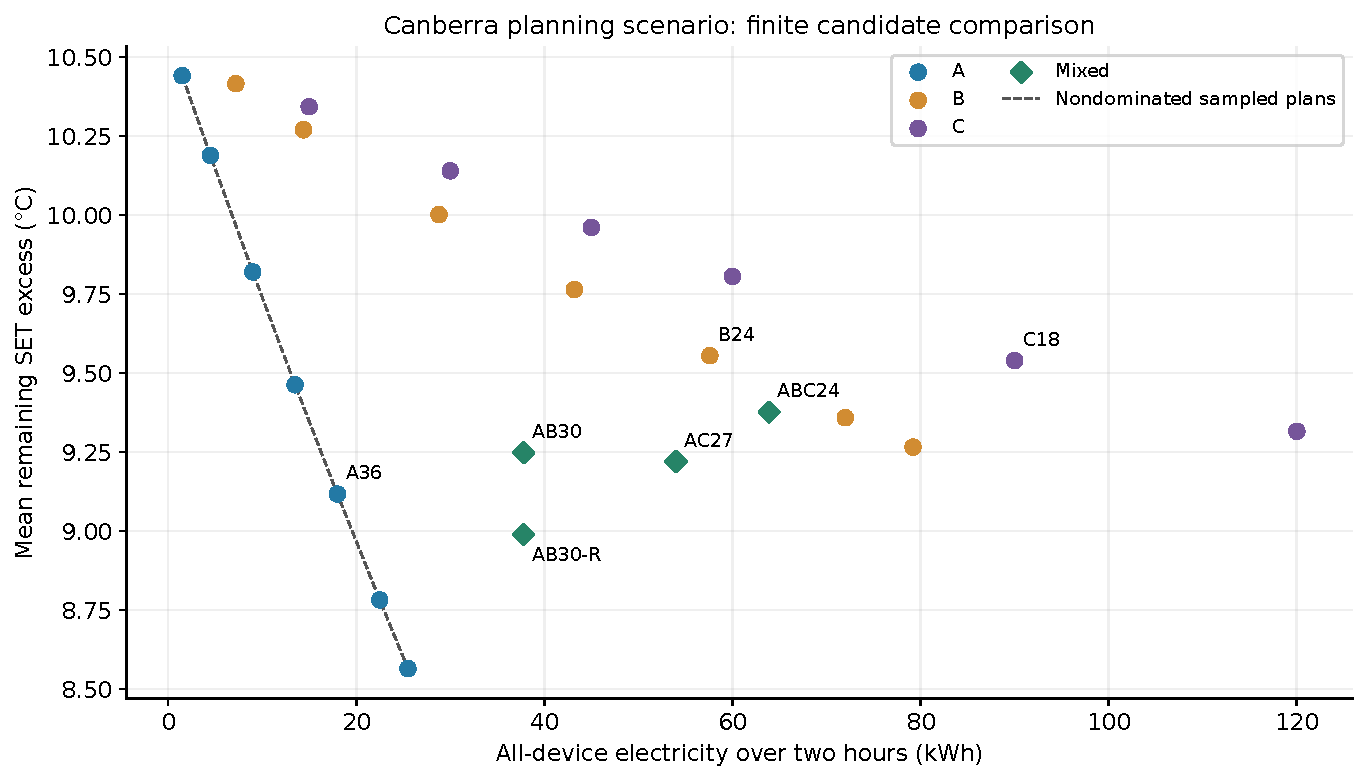
\includegraphics[width=0.86\linewidth]{figures/14_deployment_tradeoff.pdf}
\caption{Requirement 4: the quantified energy--remaining-discomfort projection. The dashed frontier concerns these two outputs of the 24 sampled plans. Experience and cost must be incorporated before claiming a four-objective frontier or an overall recommendation.}
\label{fig:effectiveness-tradeoff}
\end{figure}

The nominal energy--discomfort frontier contains A3, A9, A18, A27, A36, A45 and A51. Delivery uncertainty also matters to the performance objective: among the six equal-coverage benchmarks, AC27 leaves the least discomfort when $\chi=0$ and $\beta\ge0.5$, or when $(\beta,\chi)=(1,0.5)$, although A36 retains the highest efficiency in all 15 tested combinations. At $(0.5,0)$ their residuals are $9.02$ and $9.06\,^{\circ}\mathrm C$, while electricity is 54 and 18 kWh. The full performance/efficiency sensitivity remains available as a separate PDF in the computational material. These tradeoffs belong to overall effectiveness; the visitor-experience and cost inputs must be completed before making the final operating recommendation.
